%!TEX root = main.tex
\section{Data and Experiments}
\label{sec:data_and_experiments}

In this section, we begin by describing the
    pre-processing we did in order to use the New York City 
    Yellow taxi rides public dataset and then we
    evaluate our framework. 

\subsection{Data pre-processing}

To train our model, we need to construct the time-evolving city
    matrices - {\demandmatrix}, {\rewardmatrix}, and {\traveltimematrix} 
    described in Section \ref{sec:problem_setup}.

\spara{Hexagonal binning of New York City:}
We employ the popular methodology of hexagonal binning to discretize the city 
    into a set $\hexbins$
    of 250 non-overlapping uniform-sized hexagonal zones. 
The distance from the center of a zone to its vertices is about 1 mile.

\spara{Forming time-evolving matrices:}
We begin with the NYC Taxi dataset (2015), which contains
    street-hail records of over 200,000 taxi rides per day with information
    regarding pickup and dropoff locations and times, fare, trip distances, etc.,
    from before the significant confounding effects of ride-sharing
    platforms like Uber, Lyft, etc. 
For each ride in the dataset, we evaluate its pickup and dropoff zones
    based on location coordinates. 
Assuming that passengers do not
    hail a taxi for short distances, we ignore a small percentage of rides
    which begin and end within the same zone.

We discretize a 24-hour day into 288 time-slices of
    duration 5 minutes each, indexed by their start time. 
Thus, to populate the entries of the matrices {\demandmatrix}, {\rewardmatrix}
    and {\traveltimematrix} at time $t$, we use the rides from the dataset in the 5
    minutes time-slice beginning at time $t$. 
Due to variations in the popularity of particular pickup and dropoff
    zones at specific times of the day, the {\rewardmatrix} and
    {\traveltimematrix} matrices obtained using this
    method are sparse. 
However, to compute the best policies, our framework requires 
    the availability of complete information regarding rewards and travel times.
Hence, we estimate the missing values in these matrices using linear regression
    models including fixed-effects for the time of the day, the source and
    destination zones
\footnote{To compute the travel time entry
    $\tau(i,j)$ at time $t$, we fit a linear regression model $\tau(i,j,
    t) = \overline{\beta_0} X_{i,j,t} + \beta_1 \alpha_i + \beta_2 \alpha_j + \beta_3 \alpha_t + \epsilon_{i, j, t}$ where
    $X_{i,j,t}$ are the time-variant predictors, the $\alpha_i,
    \alpha_j$, and
    $\alpha_t$ are time-invariant fixed-effects for source, destination and
    time of the day respectively, while $\epsilon_{i,j,t}$ is standard normal error.}. 
The performance of our model is not sensitive to the
    choice of a specific linear regression modeling technique.

\subsection{Experimental results}

\subsubsection{Settings} For all experiments, we use a multiprocessor 
    implementation of our algorithm
    on a 24-core 2.9 GHz Intel Xeon E5 processor with 512 GB memory. 
The model training time for 100 episodes of training takes less than an hour. The
model testing time is less than 5 minutes. 
Our code has been made publicly available for reproducibility
purposes~\cite{github-page}.
All our experiments use learning rate $\alpha= 0.01$ and 
    discount factor $\gamma= 0.99$.
During independent learning, the exploration factor ($\epsilon$) used 
    in $\epsilon$-greedy Q-learning decreases exponentially as the 
    training progresses.
Unless mentioned otherwise, we train 5,000 drivers over 200 episodes 
    and set the imbalance threshold ({\imbalancethreshold}) to 2. 
Experimental results presented in this paper are obtained by training models 
    over a representative day viz., first Monday of September 2015 
    with a demand of over 232,000 rides.
However, our results generalize to any day. 

\subsubsection{Model performance}
First, we address the question: \textit{how well does our reinforcement
    learning-based algorithm learn the driver dispatch policy?}
In Figure~\ref{fig:rl_training}, we observe the improvement in mean driver 
    earnings and demand fulfillment as the training progresses. 
We split the 200 training episodes into independent learning episodes
    ($E_{IL}=160$) and coordinated learning episodes ($E_{CL}=60$). 
This can be achieved by setting the degree of coordination ($\xi$) to 1 until 
episode number $E - E_{CL}$ on line 9 of Algorithm~\ref{alg:general_learning}.
Consequently, episodes $[140, 160]$ utilize both independent and
    coordinated learning. 
In Figure~\ref{fig:rl_training}, we
    observe a significant improvement in the objective in the interval 
    denoted by a shaded region. 
As expected, coordinated learning appropriately relaxes some of the constraints imposed by 
    single-agent MDP and leads to significantly better performance.

In Figure~\ref{fig:model_performance}, we plot the total demand at various 
    times in the day, along with its fulfilled and unfulfilled portions
    by drivers following our policy. 
About 95\% of the total demand during the day is
    satisfied with our framework. 
We consider a ride request fulfilled if an idle driver is present in the 
    same zone at the time of the request. 
We find that 10\% of unfulfilled demand can be fulfilled by nearby drivers by adding 
    10 minutes of passenger wait, and 75\% of unfulfilled demand with 15 minutes of
    wait.
At the beginning of a day, 
for lack of better alternative, 
    we initialize drivers 
    uniformly across the city zones. 
Hence, our model requires a ``warm-up'' time for the drivers to reposition
    themselves in order to fulfill the demand. 
This warm-up interval contributes significantly to the unfulfilled
    demand at the beginning of the day from 12AM-1AM. 
One may left-pad the training interval to alleviate this issue.

The explicit coordination in our model 
    allows us to visualize the market conditions in which it is utilized.
In Figure~\ref{fig:wait_probability}, we plot snapshots of
    coordination in form of a heatmap with probabilities of 
    coordinated wait actions i.e. $Q_C(t, h, h)$ at 6 AM during the early 
    morning commute and at 6 PM during the evening commute\footnote{More
    detailed visualizations depicting evolution of coordinated actions and degree of
    coordination across the city and through the time of the day are available 
    at~\cite{github-page}.}.
Without coordination, we would expect all the drivers in the city to relocate
    to Manhattan in order to satisfy the extremely high volume of demand during
    the morning commute. 
However, as observed in Figure~\ref{fig:wait_probability},
    our model recommends a certain proportion of drivers to wait in the outer
    boroughs of New York City for the early morning commute to Manhattan.
Notably, the model is able to learn demand trends in time-dependent hotspots
    such as the J.F.K. airport to the south-east of the city.
In contrast, during the evening commute to outer boroughs, the model 
    strongly recommends
    that the drivers wait inside Manhattan.

\begin{figure}
	\centering
    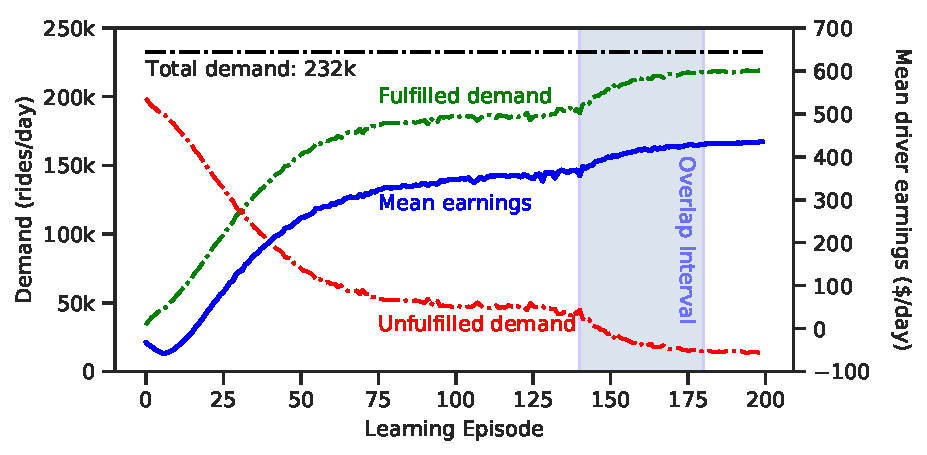
\includegraphics[scale=0.5]{figures/rl_training.pdf}
	\caption{A representative illustration of improvement in mean driver 
    earnings during training.} 
	\label{fig:rl_training}
\end{figure}

\begin{figure}[h]
    \centering
    \begin{tabular}{ c }
        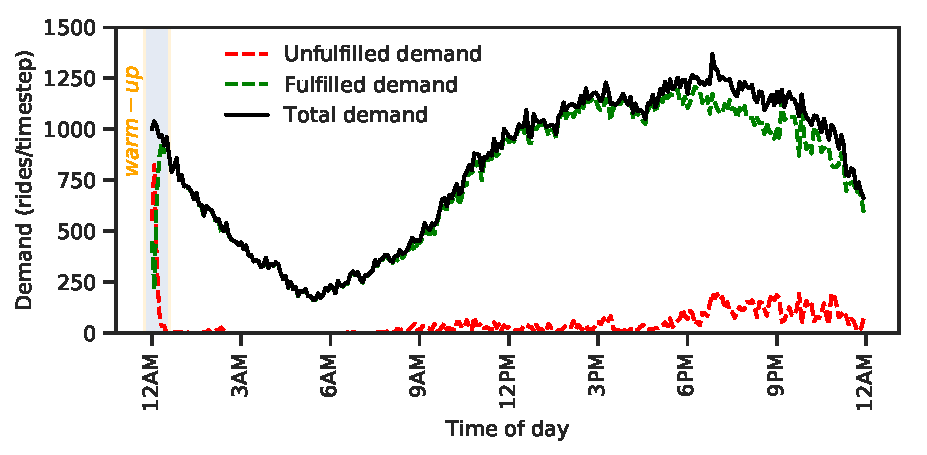
\includegraphics[scale=0.5]{figures/model_performance.pdf} \\
        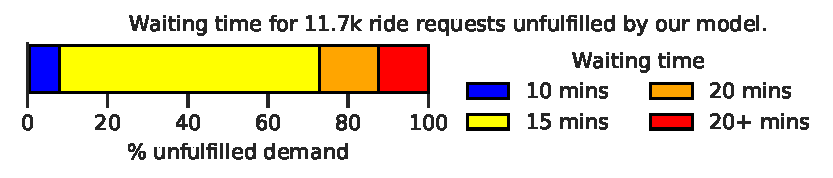
\includegraphics[scale=0.5]{figures/pax_waiting_time.pdf}
    \end{tabular}
    \caption{Top: Demand fulfillment by a trained policy at different times on a representative
        day. Bottom: Waiting times for demand not immediately fulfilled by the model.}
    \label{fig:model_performance}
\end{figure}

\begin{figure*}[h]
    \centering
    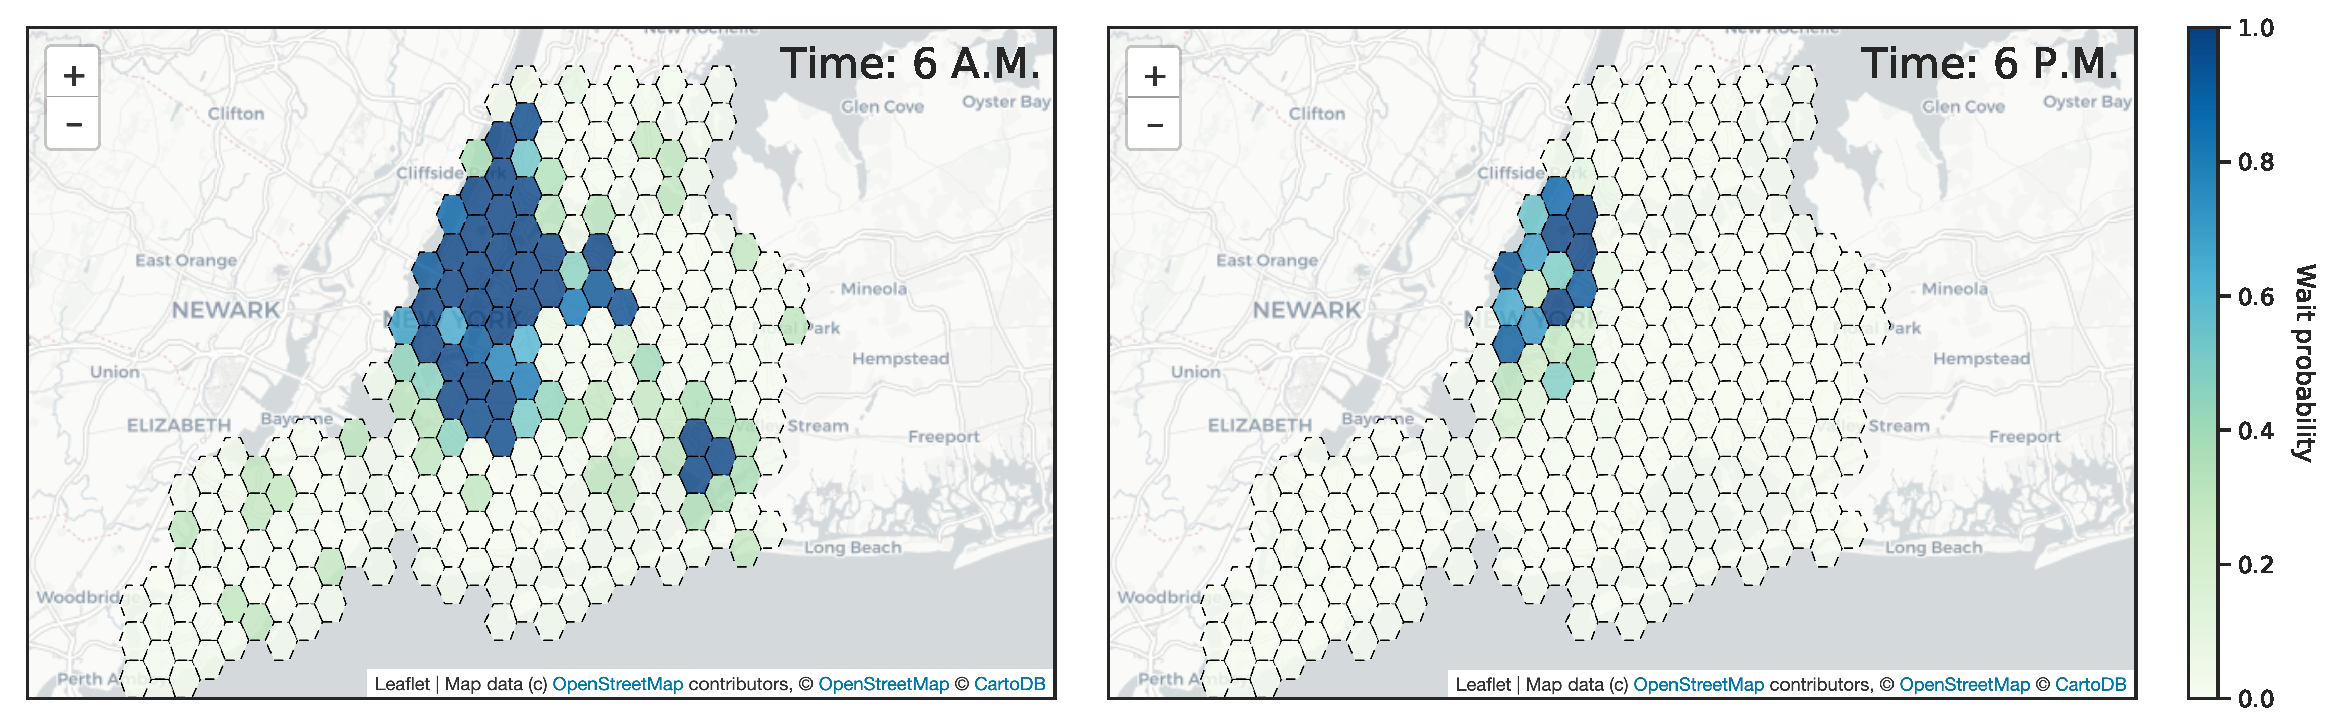
\includegraphics[width=12cm, height=3.5cm]{figures/wait_probability.pdf}
    \caption{
        Heatmaps of probability of coordinated wait i.e., $Q_C(t, h, h)$ during
        morning commute at 6 A.M. (left) and evening commute at 6 P.M. (right).
        }
    \label{fig:wait_probability}
\end{figure*}

\subsubsection{Impact of independent and coordinated learning}
The overlap between the independent 
    and the coordinated learning during training is a crucial 
    aspect of our framework.
In this section, we address the question:
    \textit{how do we determine
    the appropriate number of independent learning and coordinated learning
    episodes during training?}
Given a fixed number of training episodes $E$, we assume that 
    our model trains the initial $E_{IL}$ episodes with independent learning 
    and the final $E_{CL}$ episodes with coordinated learning. 
When $E_{IL} + E_{CL} \geq E$, we have $E_{IL} + E_{CL} - E$ episodes of overlap
    between independent and coordinated learning.
In Figure~\ref{fig:il_cl_overlap}, we use 200 episodes of training, and 
    we vary the values of $E_{IL}$ and $E_{CL}$ in the range $[20,200]$ to
    achieve various overlaps\footnote{Note that there is no overlap between 
    the independent and the coordinated learning phases
in the lower triangle of Figure~\ref{fig:il_cl_overlap} when $E_{IL} + E_{CL} < E$.}.
We then plot the mean driver earnings for each learned policy.
We show that for a large interval of values of $E_{IL}$ and $E_{CL}$, 
    our framework provides stable and high performance with up to
    \$535 mean earnings per day when $E_{IL}=60$ and $E_{CL}=160$,
    denoted by a green marker in the figure.
This observation supports our claim that our framework is robust to
    imperfections in hyperparameter tuning.
Note that we have used different values of $E_{IL}$ and $E_{CL}$ in
    Figure~\ref{fig:rl_training} in order to clearly portray the incremental
    impact of coordinated learning on mean driver earnings per day.


\begin{figure}
	\centering
    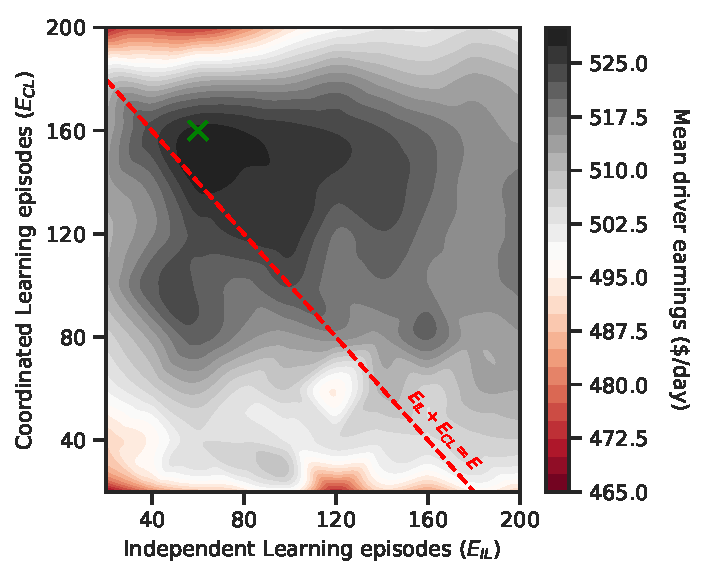
\includegraphics[scale=0.5]{figures/il_cl_overlap_200_episodes.pdf}
    \caption{Performance stability over a wide range of overlaps between the
    independent and the coordinated learning.}
	\label{fig:il_cl_overlap}
\end{figure}

\subsubsection{Impact of Driver Supply} 

We next answer the question: \textit{what is an appropriate number of drivers
    to fulfill the ride demand?}
To study this question, we vary the driver supply in the
    range $[1000, 6000]$, where the units are individual drivers. 
Given a fixed supply size, we plot the ratio of the number of successful driver 
    waits resulting into passenger rides to the number of unsuccessful driver 
    waits while taking into account the overall demand fulfillment.
When the number of drivers is small compared to the demand, the
    drivers should have an easier time finding a passenger. 
On the other hand, a city saturated with drivers should result in a 
    higher number of unsuccessful driver waits.
\begin{figure}
	\centering
	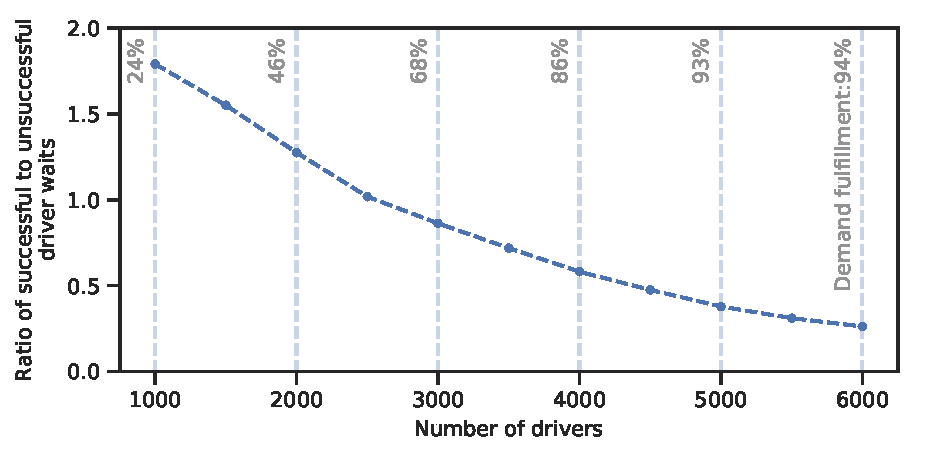
\includegraphics[scale=0.5]{figures/number_of_drivers_2.pdf}
	\caption{Impact of supply size on the ease of finding a
    passenger on a representative day.}
	\label{fig:number_of_drivers}
\end{figure}
In Figure~\ref{fig:number_of_drivers}, we observe that the framework validates
    our expectations.
The ``warm-up'' period described in Figure~\ref{fig:model_performance}
    causes underestimation of demand fulfillment while it simultaneously
    causes overestimation of 
    the number of unsuccessful driver waits. 
Excluding the warm-up interval, this experiment provides evidence that over 96\%
% \footnote{Excluding the
%     warm-up interval from the analysis improves the demand fulfillment to 96\%.} 
    demand of 
    New York City can be fulfilled by about 5,000 drivers. 
Note that in September 2015, New York City had over 
    13,500 operational taxicab medallions~\cite{wiki-001}. 
It also justifies our decision to use 5,000 drivers in most of our experiments. 


\subsubsection{Impact of platform objectives}
So far, our experiments focused on the \textsc{MaxEarnings} problem.
A natural question is: \textit{should a platform optimize driver dispatches to maximize their earnings 
    or to maximize demand fulfillment?}
Note that while maximizing the demand fulfillment might help retain customers 
    over a longer-term, it can
    be detrimental to drivers' earnings.
\begin{figure}
	\centering
	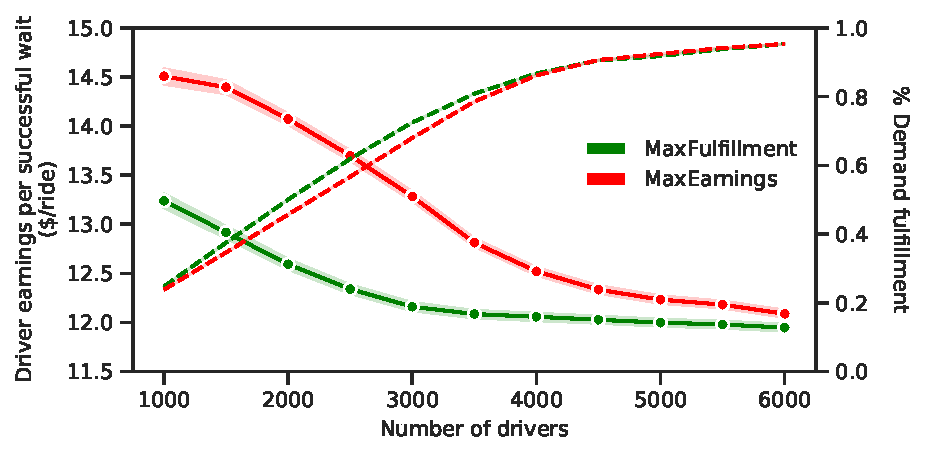
\includegraphics[scale=0.5]{figures/pickups_vs_revenue_objective_2.pdf}
    \caption{Differential impact of platform objectives.
    Left Y-axis: Driver earnings per passenger ride 
    with 90\% confidence interval.
    Right Y-axis: \% Demand fulfillment for both objectives on a 
    representative day.}
	\label{fig:pickups_vs_revenue_objective}
\end{figure}
To solve \textsc{MaxFulfillment} (see Section~\ref{sec:problem_setup}),
the framework rewards (resp.\ penalizes) a
successful passenger pickup (resp.\ unsuccessful wait) by +1 (resp.\ -1)
net reward.
Figure~\ref{fig:pickups_vs_revenue_objective} depicts that mean driver earnings 
    per passenger ride can be over a \$1 lower in a policy optimized for 
    maximizing demand fulfillment relative to one optimized for earnings.
The additional rides covered by the solution to \textsc{MaxFulfillment} may  
    direct drivers to sub-optimal locations
    and compromise their future earnings for the day.
As the supply increases over the minimum number of required drivers, the 
    two objectives converge while a statistically significant difference in 
    the driver earnings per ride persists.
Note that higher rewards/penalties while solving 
    \textsc{MaxFulfillment} result in larger divergence between the 
    two objectives.

\subsubsection{Advantage of strategic behavior}
Next, we address the question: \textit{does our model provide consistently
    higher earnings for all the drivers?}
To explore this, we model the taxi driver population of the city as comprised
    of strategic drivers who follow the model recommendations and naive drivers
    who act upon heuristics learned via experience. 
We expect the mean earnings of drivers to decrease as the number of
    strategic drivers on the platform increases.
While modeling a naive driver, we assume that taxi drivers, over time, 
    learn the popular spots in the city. 
If they are unable to locate passengers reasonably quickly 
    in other parts of the city, they head back to the popular spots. 
    We designate 15 zones %in Lower Manhattan, J.F.K Airport, Newark Airport, etc.
    as
    popular zones based on the historical demand data.
Furthermore, we assume that an idle naive driver looking for a passenger decides to 
    head back to one of the popular zones with a fixed probability of 0.25. 
Upon choosing to relocate, the naive driver picks the target popular zone with a 
    probability inversely proportional to its distance from the current location.

\begin{figure}
	\centering
	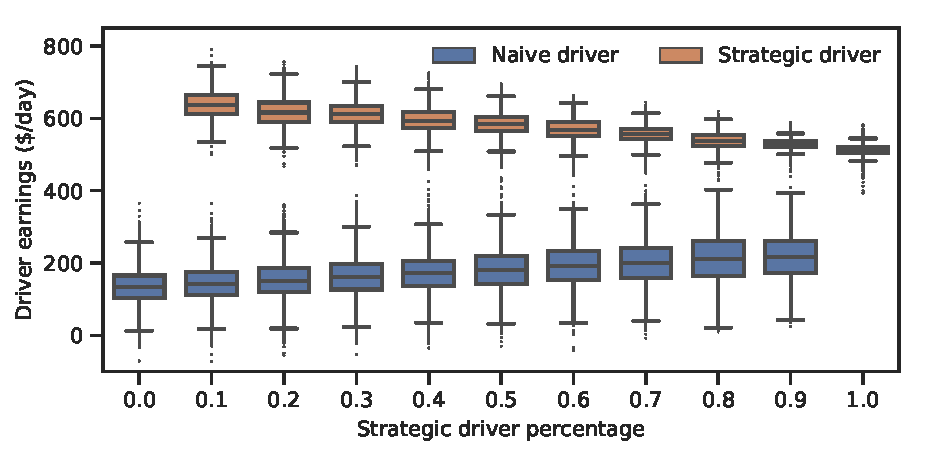
\includegraphics[scale=0.5]{figures/strategic_vs_naive_driver.pdf}
    \caption{Earnings advantage of the strategic drivers over the naive drivers 
    on a representative day.} 
	\label{fig:strategic_vs_naive_driver}
\end{figure}

In Figure~\ref{fig:strategic_vs_naive_driver}, we plot the earnings of
    the two categories of drivers while varying the percentage of
    strategic drivers.
% \footnote{The lower and upper edges of the boxes in
%     Figure~\ref{fig:strategic_vs_naive_driver} indicate quartiles Q1 and Q3
%     respectively, and the length of whisker is 1.5 times IQR.}. 
As expected, an increase in the number of strategic drivers causes their individual 
    earnings to decline. %-- `price of anarchy'. 
Overall, the strategic drivers not only earn more than the naive
    drivers, but also the variance in their earnings is significantly lower.
Thus, our framework is \emph{envy-free}, i.e., drivers at the same
    location and time do not envy each other's future earnings.

\subsubsection{Model generalizability}
\label{sec:model_generalizability}
\begin{figure}
	\centering
    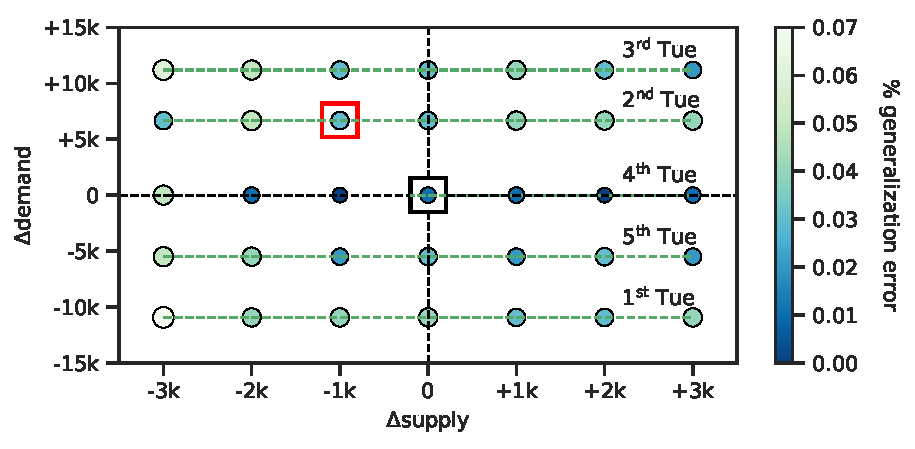
\includegraphics[scale=0.5]{figures/model_generalizability_2.pdf} 
    \caption{Model robustness: Baseline model 
    (enclosed within a black box at origin) is 
    deployed on other Tuesdays.} 
	\label{fig:model_generalizability}
\end{figure}
In this section, we explore the question of model generalizability: 
    \textit{does our
    model perform well when deployed on days with considerably different supply-demand conditions 
compared to the day it was trained on?}
We cross-validate our model by evaluating the policy of a trained model on different days. 


For illustrative purposes, we choose as baseline --
    $m_0$ -- a model
    trained to satisfy the demand of 288,000 rides observed on
    the fourth Tuesday of September using 7,000 drivers. 
We test the policy $\pi(m_0)$ recommended by our 
    baseline model by deploying it on other Tuesdays of the month. 
Note that the observed demand, as well as the number of active drivers might
    vary on other Tuesdays compared to
    our baseline model. 
To capture this potential for change in supply, we vary the number of
    simulated drivers during testing in the range $[4000, 10000]$.
In Figure~\ref{fig:model_generalizability}, enclosed within a red square box is
    an illustration of the generalization error associated with deploying our
    baseline model's recommended policy on the second Tuesday of the month with
    just 6,000 drivers.
Importantly, the policy $\pi(m_0)$ now attempts to fulfill an increased 
    demand of about 7,000 extra rides ($\Delta demand$) using 1,000 fewer drivers 
    ($\Delta supply$) than it was trained for.
To evaluate its performance in this task, we compare it with a model
    $m_*$ which was explicitly trained to fulfill the demand of
    the second Tuesday with exactly 6000 drivers.
Thus, we compute the baseline policy's generalization error as
    \begin{equation*}
        \% \textrm{generalization error} =
        \frac{\mathcal{F}^{\pi}(m_*)-\mathcal{F}^{\pi}(m_0)}
        {\mathcal{F}^{\pi}(m_*)},
    \end{equation*}
    where $\mathcal{F}^{\pi}(m)$ denotes the demand fulfillment of model $m$.

Figure~\ref{fig:model_generalizability} shows that our framework
    generalizes well to perturbations in both supply and demand. 
We also observe that decreasing the number of drivers excessively 
    impacts harms its generalization performance. 
As a result, we recommend deploying models trained with a reasonably higher 
    number of drivers than minimally required so that they generalize better in 
    cases of varying demand. %scenarios.
For brevity, we have presented a single illustrative example here; 
    the generalizability result holds true across all the models.

\subsubsection{Comparison with baselines}
\label{sec:comparative_baselines}
\begin{figure}
	\centering
	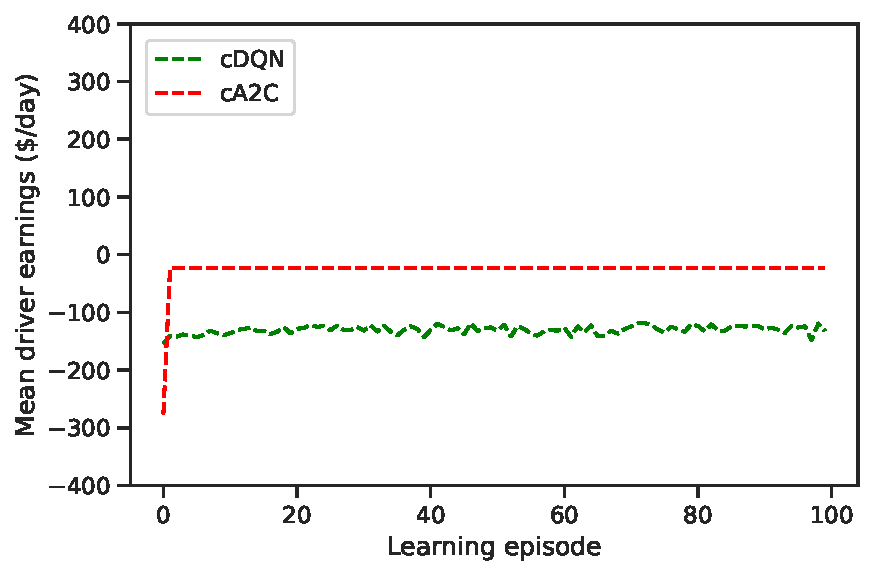
\includegraphics[scale=0.36]{figures/comparative_baselines.pdf}
    \caption{Performance of cDQN and cA2C deep-learning approaches from ~\cite{Lin2018-vs}.} 
	\label{fig:comparative_baselines}
\end{figure}
A major challenge in comparative studies in this domain is the
    lack of reproducibility due to proprietory datasets and
    simulators.
To the best of our knowledge, although~\cite{Lin2018-vs} uses coordinated deep
    reinforcement learning approach, it is most similar to 
    ours with respect to modeling assumptions. 
In the absence of the  Didi Chuxing's proprietary driver 
    simulator and datasets, direct comparison of our works is impossible. 
We make an effort to compare our approaches by re-implementing their deep 
    reinforcement learning based algorithms (cDQN and cA2C) with minimal 
    modifications to fit 
    our setting which computes future driver distributions based on simulating
    passenger pickups and dropoffs, instead of predicting them using proprietary
    models.
    
In~\cite{Lin2018-vs}, the authors do not train the neural network
    from its randomly initialized state.
Instead, they bootstrap the network based on a \textit{pre-trained value networks
    based on historical means} from the aforementioned simulator.
As a direct and fair comparison with our model which does not rely on
    external pre-trained inputs, our implementations of their algorithms 
    also attempt to learn \emph{from scratch}. 

Figure~\ref{fig:comparative_baselines} shows mean driver earnings per day over
    the course of model training.
Even after extensive hyperparameter tuning, the baselines failed
    to learn meaningful strategies, with driver earning net negative rewards
    of -\$20 over a day.
In the absence of a pre-trained value network, the
    algorithms proposed in~\cite{Lin2018-vs} are unable to explore the policy space
    effectively.
Moreover, the reward sharing assumption used in~\cite{Lin2018-vs} results in a 
    superficial coordination behavior which fails to learn in a more realistic 
    scenario such as ours, which simulates actual passenger pickups and dropoffs.
Our implementations of contextual DQN (cDQN) and contextual actor-critic (cA2C)
    algorithms
    % with an extensive conceptual comparison with our framework 
    are publicly available at \cite{github-page}. 
